\documentclass[11pt]{article}
\usepackage[a4paper,margin=2.5cm]{geometry}
\usepackage[T1]{fontenc}
\usepackage{lmodern}
\usepackage{graphicx}
\usepackage{booktabs}
\usepackage{amsmath}
\usepackage{hyperref}
\usepackage{xcolor}

\title{Telling Stylized Avatars Apart at a Glance:\\Contour Height Maps and Silhouette Overlap for Hairstyle Design in Shared XR}
% Author as the owner chose it (arXiv lists authors publicly).
\author{Y.T.\\\small Independent researcher}
\date{}

\begin{document}
\maketitle

\begin{abstract}
In shared extended reality (XR), people meet many avatars at once and often see them small, far away or from behind.
Stylized ``cute'' faces make this harder: the cues that make a face read as cute (a round outline, a large forehead, a small nose and chin) also make faces resemble one another.
We describe a small, reproducible design method that separates the two jobs.
Faces are modelled as height maps and studied through their contour lines, built from a reference face step by step (outline, masses, nose and brow, mouth and chin, hairline).
Distinguishability is measured as the intersection-over-union (IoU) of binary silhouettes.
For four stylized figures, faces alone overlap with IoU $0.87$--$0.95$; giving each figure one dominant hairstyle silhouette (ponytail, bob, two buns, cloud) lowers every pair to $0.62$--$0.73$.
Texture-like styles such as braids barely change the silhouette (IoU $0.87$ against no hair) and work as a second layer, not as the dominant shape.
All numbers and figures are produced by an open script from the same code as an interactive tool.
\end{abstract}

\section{Introduction}
Shared, social XR---the ``eXtended meta/uni/Verse'' (XV) in the terminology of Mann et al.~\cite{mann2022xv}---puts many avatars in one view.
Recognising who is who at a glance matters there in a way it does not for a single character on a screen.
Character designers often check this with a ``squint test'': shrink the character until only its filled silhouette is left, and see whether it can still be told apart from the others.

This note turns that habit into a number and applies it to a specific tension.
Stylized avatars are frequently designed to look cute.
The baby-schema cues associated with cuteness~\cite{lorenz1943,glocker2009}---a rounder face, a larger forehead, a small nose and chin---push faces toward one shared shape.
We show, on a deliberately simple model, how much this costs in distinguishability and how a single dominant hairstyle per figure buys it back.

Our contributions are modest and practical:
(i) a height-map face model whose personality is added coarse to fine, so each step can be inspected as a change in contour lines;
(ii) a silhouette-overlap measure and a working threshold for ``too similar'';
(iii) measurements for four stylized figures and eight hairstyle types; and
(iv) an open, reproducible script.

\section{Method}
\subsection{Faces as height maps}
A face is a height map $z(x,y)$: a dome of half-width $r_x$ and half-height $r_y$, $z_0 = 0.9\sqrt{1 - (x/r_x)^2 - (y/r_y)^2}$, plus Gaussian bumps for forehead, cheeks, jaw, brow, eye sockets, nose, mouth and chin, and a plateau above the hairline.
The heights are a drawing model, not anatomy.
Personality is added in five steps, from wide contour spacing to narrow: (1) outline $(r_x, r_y)$; (2) masses (forehead, cheeks, jaw); (3) nose and brow; (4) mouth and chin; (5) hairline.
At step $s$ a face uses its own parameters for steps $\le s$ and the reference face's for the rest, so the difference map $\Delta z = z_\text{face} - z_\text{ref}$ shows each layer arriving.
Contour lines are extracted with marching squares, the two-dimensional case of marching cubes~\cite{lorensen1987}; the two saddle cases are resolved by the cell's centre value.

\subsection{Hair as height on the same map}
Hair is added to the same height map rather than placed as a separate object: a tower above the crown, horizontal wings at temple height, a bob as a helmet-shaped plateau with a fringe, braids as narrow ridges, a ponytail as a tapered tube from the crown past the shoulder, two ring-shaped buns, and a cloud whose rim wobbles with two sine terms.
A detail layer adds the parts that vary most between styles: the fringe type (blunt, swept, covering one eye, see-through), the parting ratio, and the lengths of the left and right side locks.
The head is sampled on a $90\times110$ grid over $x\in[-1.35,1.35]$, $y\in[-1.3,1.75]$.

\subsection{Silhouette overlap}
A silhouette is the set of grid cells with $z > 0.02$.
For two silhouettes $A$ and $B$ aligned on the same grid, distinguishability is measured by the Jaccard index~\cite{jaccard1912}, $\mathrm{IoU}(A,B) = |A\cap B| / |A\cup B|$; $1$ means identical.
We use $\mathrm{IoU} \ge 0.75$ as a working flag for ``too similar''.
This threshold is a design heuristic chosen from inspecting the small filled silhouettes, not a perceptual result.

\section{Results}
\subsection{Cute faces converge}
Table~\ref{tab:outline} lists the outlines of the four figures; each keeps one outline cue of its own (round, roundest and shortest, slim oval, heart-shaped).
Still, with faces alone every pair overlaps strongly, with IoU between $0.87$ and $0.95$ (Table~\ref{tab:four}, grey bars in Fig.~\ref{fig:iou}, top row of Fig.~\ref{fig:sil}).

\begin{table}[htbp]
\centering
\begin{tabular}{lccc}
\toprule
Figure & $r_x$ & $r_y$ & $r_y/r_x$ \\
\midrule
Ponytail & 0.84 & 0.98 & 1.17 \\
Bob & 0.83 & 0.94 & 1.13 \\
Buns & 0.74 & 1.04 & 1.41 \\
Cloud & 0.80 & 1.00 & 1.25 \\

\bottomrule
\end{tabular}
\caption{Face outlines (step 1). Figures are named by their dominant hairstyle.}
\label{tab:outline}
\end{table}

\subsection{One dominant hairstyle per figure}
Giving each figure a different dominant hairstyle (ponytail, bob, buns, cloud) plus its detail layer lowers every pair below the flag, to $0.62$--$0.73$ (Table~\ref{tab:four}, black bars in Fig.~\ref{fig:iou}; contours in Fig.~\ref{fig:contours}).
An earlier assignment in which two figures both had round masses (bob and cloud) left that pair at $0.81$; separating them by direction---a flat, low helmet against a cloud raised above the crown---resolved it.
In practice, dominant shapes are easiest to separate when they differ in direction: round, tall, wide, or off to one side.

\begin{table}[htbp]
\centering
\begin{tabular}{llcc}
\toprule
\multicolumn{2}{c}{Pair} & Face only & With hair \\
\midrule
Ponytail & Bob & 0.95 & 0.70 \\
Ponytail & Buns & 0.88 & 0.68 \\
Ponytail & Cloud & 0.95 & 0.66 \\
Bob & Buns & 0.87 & 0.62 \\
Bob & Cloud & 0.94 & 0.65 \\
Buns & Cloud & 0.92 & 0.73 \\

\bottomrule
\end{tabular}
\caption{Silhouette IoU for every pair of the four figures.}
\label{tab:four}
\end{table}

\begin{figure}[htbp]
\centering
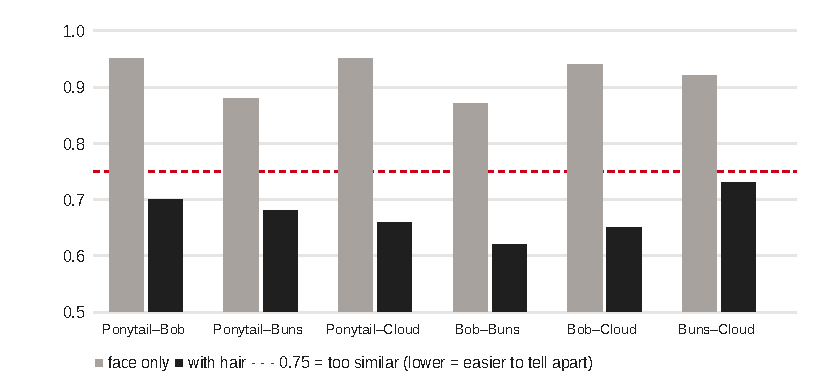
\includegraphics[width=0.85\linewidth]{figures/fig3-iou.pdf}
\caption{IoU per pair: faces only (grey) and with hair (black). The dashed line marks the working threshold $0.75$.}
\label{fig:iou}
\end{figure}

\begin{figure}[htbp]
\centering
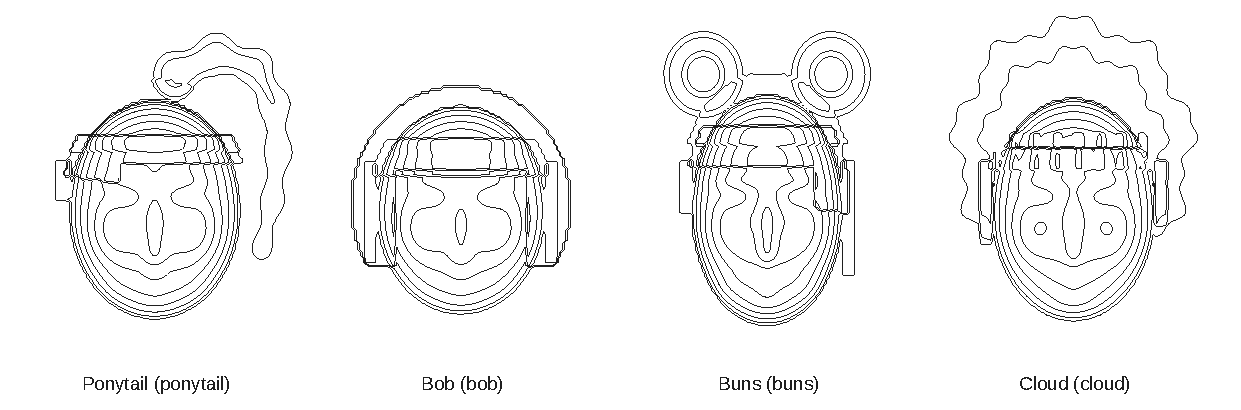
\includegraphics[width=0.95\linewidth]{figures/fig1-contours.pdf}
\caption{Contour lines of the four figures with hair (ten levels each).}
\label{fig:contours}
\end{figure}

\begin{figure}[htbp]
\centering
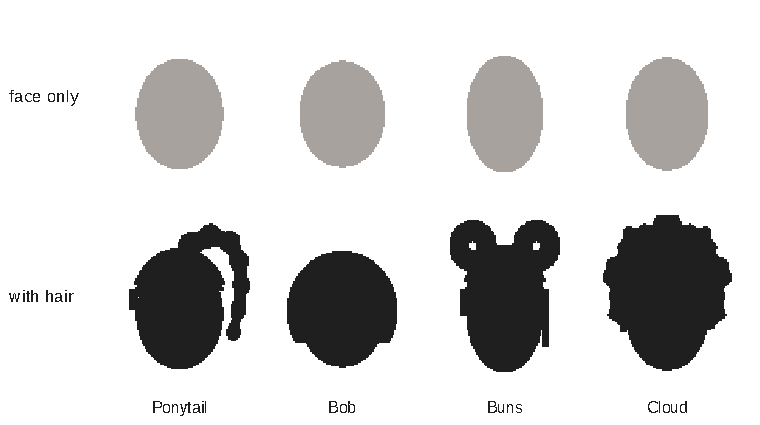
\includegraphics[width=0.7\linewidth]{figures/fig2-silhouettes.pdf}
\caption{The squint test: filled silhouettes, faces only (top) and with hair (bottom).}
\label{fig:sil}
\end{figure}

\subsection{Dominant shapes and textures}
Fig.~\ref{fig:matrix} isolates the hair: every style on the same reference face.
Braids overlap a bare head at $0.87$ and wings at $0.87$: they change the surface, not the outline, and are better used as a second, texture layer.
The cloud is the most distinct from a bare head ($0.52$).
Variants of one style behave the same way (Table~\ref{tab:bob}): a blunt cut that widens the outline ($0.76$ against the plain bob) or an asymmetric cut ($0.84$) changes the silhouette, while an inward curl or layering ($0.92$) mostly does not.

\begin{figure}[htbp]
\centering
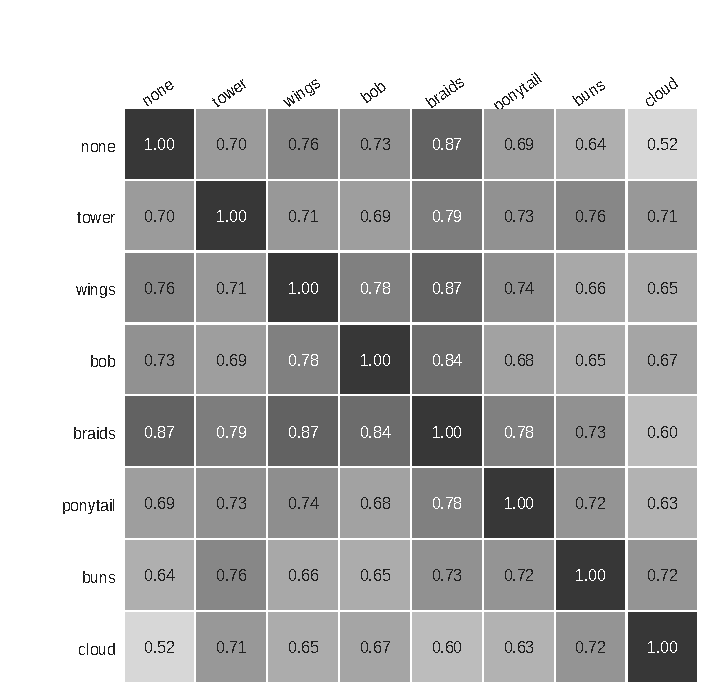
\includegraphics[width=0.6\linewidth]{figures/fig4-style-matrix.pdf}
\caption{IoU between hairstyles on the same reference face (darker = more alike).}
\label{fig:matrix}
\end{figure}

\begin{table}[htbp]
\centering
\begin{tabular}{lc}
\toprule
Bob variant & IoU vs.\ plain bob \\
\midrule
\texttt{bob-asym} & 0.84 \\
\texttt{bob-inward} & 0.92 \\
\texttt{bob-blunt} & 0.76 \\
\texttt{bob-layer} & 0.92 \\

\bottomrule
\end{tabular}
\caption{Variants of one style: which ones change the silhouette.}
\label{tab:bob}
\end{table}

\section{Discussion and limitations}
The measure is deliberately crude.
Silhouettes are taken from the front only, while avatars in XR are seen from every side; the next step is to average IoU over many viewpoints (for example, 22 cameras on a ring at three heights).
The face model is a sum of smooth bumps, not anatomy.
The $0.75$ threshold has not been validated with people; a small recognition study (match a silhouette to a figure, under time pressure) would turn it into a perceptual result.
Colour, which also separates avatars, is deliberately left out so that shape alone is tested.

\section{Reproducibility}
All numbers, tables and figures in this note are generated by \texttt{scripts/paper-figures.mjs} from the same code (\texttt{lib/faceContour.ts}) as an interactive tool in which the steps, hairstyles, fringe ratios and side locks can be changed and the IoU table updates live.

\bibliographystyle{plain}
\bibliography{refs}
\end{document}
